\subsection{Appraisal theory}

One of the most used models of emotions is the OCC model from \cite{ortony1990cognitive}. It is widely used in artificial intelligence and robotics and created based on the ideals of the appraisal theory. The structuring of the emotion is made in respect to the cognition of an individual, that is, how he perceives the world around him. The authors created this theory with intent to be ``computationally tractable model of emotion"\cite{ortony1990cognitive}, to be possible for a computing construct, such as an artificial intelgence system to reason on emotion \citep{ortony1990cognitive}.

The OCC model introduces the structure of emotion, that is, how an emotion emerges and what valence it has. This structure is illustrated in \autoref{fig:OCCDIagram} and thoroughly explained in the remainder of this section. 
\begin{figure}[p]
    \centering
    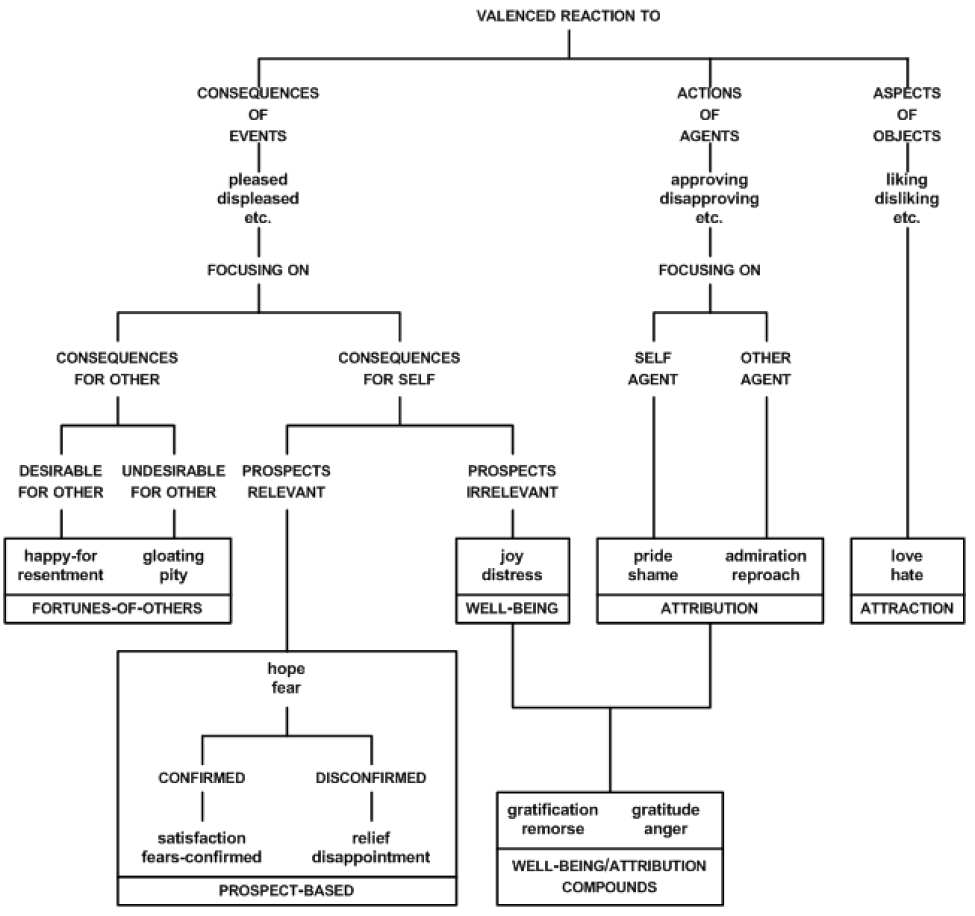
\includegraphics[width=\textwidth,height=0.7\textheight]{Images/OCCDEsenho.png}
    \caption{OCC model diagram copied from \cite{ortony1990cognitive} page 19}
    \label{fig:OCCDIagram}
\end{figure}

In accord to the appraisal theory this model starts its structure with a valenced reaction and then evaluates the focus of such reaction. There is three possible aspects of the world in which is possible to focus, consequences of events, actions of agents and aspects of objects, the first classification that is made for a valenced reaction. From this point the model dissects other possible focuses which structure the notion of the emotion types. The named boxes at the bottom of the diagram are the emotion types that categorizes emotions
